\section{The Lifecycle of a Decentralized Software Update}
%A \emph{software update (SU)} is the unit of change for the blockchain software. It must have a clear goal of what it tries to achieve and why it would be beneficial, if applied to the system. Moreover, it should have a clear scope. In Figure \ref{lifecycle}, we depict the full lifecycle of a software update following a decentralized approach. In this lifecycle, we identify four distinct phases: a) the \emph{ideation phase}, b) the \emph{implementation phase}, c) the \emph{approval phase} and d) the \emph{activation phase}. In this section, we briefly outline each phase and at the subsequent sections, we provide all necessary details for realizing each phase in a decentralized setting.
A \emph{software update (SU)} is the unit of change for the blockchain software.In Figure \ref{lifecycle}, we depict the full lifecycle of a software update following a decentralized approach.In this lifecycle, we identify four distinct phases: a) the \emph{ideation phase}, b) the \emph{implementation phase}, c) the \emph{approval phase} and d) the \emph{activation phase}.In the subsequent sections, we provide all necessary details for realizing each phase in a decentralized setting.

%The SU starts from the ideation phase which is the conceptualization step in the process. It is where an SU is born. During this phase, a justification must be made for the SU and this has to be formally agreed by the community (or the code owner). This justification takes the form of an improvement proposal document (appears as \emph{SIP} in the figure and will be defined shortly). Once the SU's justification has been approved, then we enter the implementation phase. It is where the actual development of the SU takes place. The result of this phase is a bundle \emph{update proposal (UP)} consisting of source-code (implementing the SU), metadata and optionally binaries produced for one, or more, specific platforms. This is submitted for approval and thus the approval phase follows. Once the UP has been approved (by the community, or the code owner), the community is called for upgrading. The actual upgrading takes place in the activation phase, which is there to guard against chain-splits by synchronizing the activation of the changes.

Interestingly, the phases in the lifecycle of a SU are essentially independent from the approach (centralized or decentralized) that we follow. They constitute intuitive steps in a software lifecycle process that starts from the initial idea conception and ends at the actual activation of the change on the client software. Based on this observation, one can examine each phase and compare the traditional centralized approach, used to implement it, to its decentralized alternative. In the appendix you can find a description of the centralized approach for each phase, for comparison reasons. Moreover, not all phases need to be decentralized in a real world scenario. One has to measure the trade-off between decentralization benefits versus practicality and decide what phases will be decentralized. Our decomposition of the lifecycle of a SU in distinct phases helps towards this direction.

\begin{figure}[h!] %[H]
    \caption{The lifecycle of a software update (a decentralized approach)}
    \centering
%    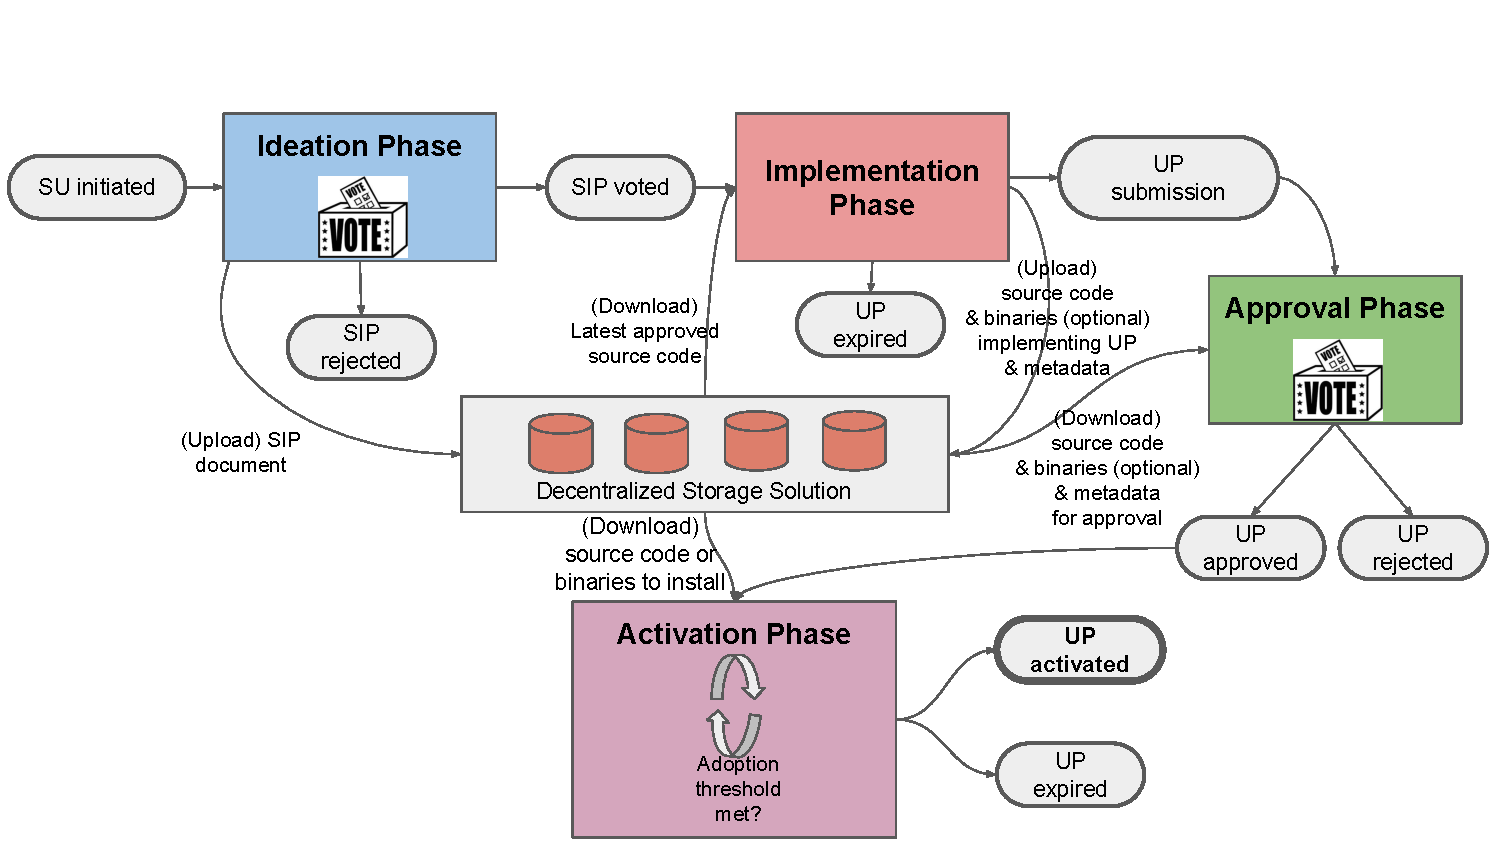
\includegraphics[width=\textwidth]{figures/lifecycle_phases.pdf}
    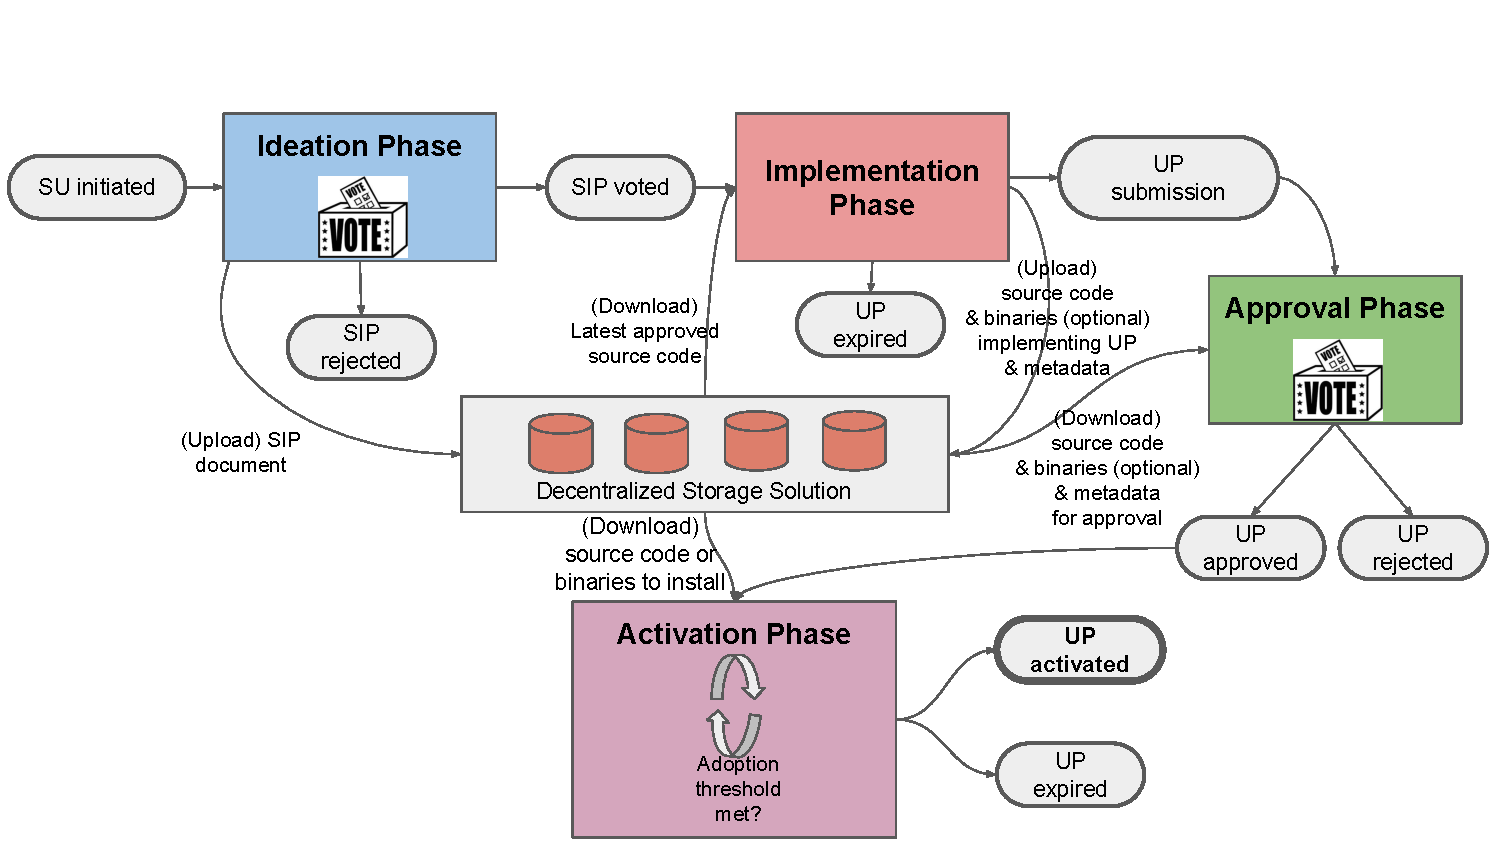
\includegraphics[width=1.0 \columnwidth,keepaspectratio]{figures/lifecycle_phases.pdf}
    \label{lifecycle}
\end{figure}

\subsection{Ideation}
%\paragraph{Scope of the phase.} 
A SU starts as an idea. Someone captures the idea of implementing a change that will serve a specific purpose (fix a bug, implement a new feature, provide some change in the consensus protocol, perform some optimization etc.). The primary goal of this phase is to capture the idea behind a SU, then record the justification and scope of the SU in some appropriate documentation and finally come to a decision on the priority that will be given to this SU. 

%\paragraph{Centralized approach.}
%Traditionally, in the centralized approach, a SU is proposed by some central authority (original author, group of authors, package maintainer etc.), who essentially records the need for a specific SU and then decides when (or, in which version) this could be released. In many cases, (e.g., Bitcoin \cite{bitcoin}, Ethereum \cite{ethereum}) the relevant SU justification document (called BIP, or EIP respectively) is submitted to the community, in order to be discussed. Even when this \say{social alignment} step is included in this phase, the ultimate decision (which might take place at a later phase in the lifecycle), for the proposed SU, is taken by the central authority. Therefore, the road-map for the system evolution is effectively decided centrally. Moreover, this social consensus approach is informal (i.e., not part of a protocol, or output of an algorithm) and is not recorded on-chain as an immutable historical event.

%\paragraph{Decentralized approach.}
The ideation phase in the decentralized approach is depicted in Figure \ref{ideation}.
\begin{figure}[h!] %[H]
    \caption{The ideation phase.}
    \centering
    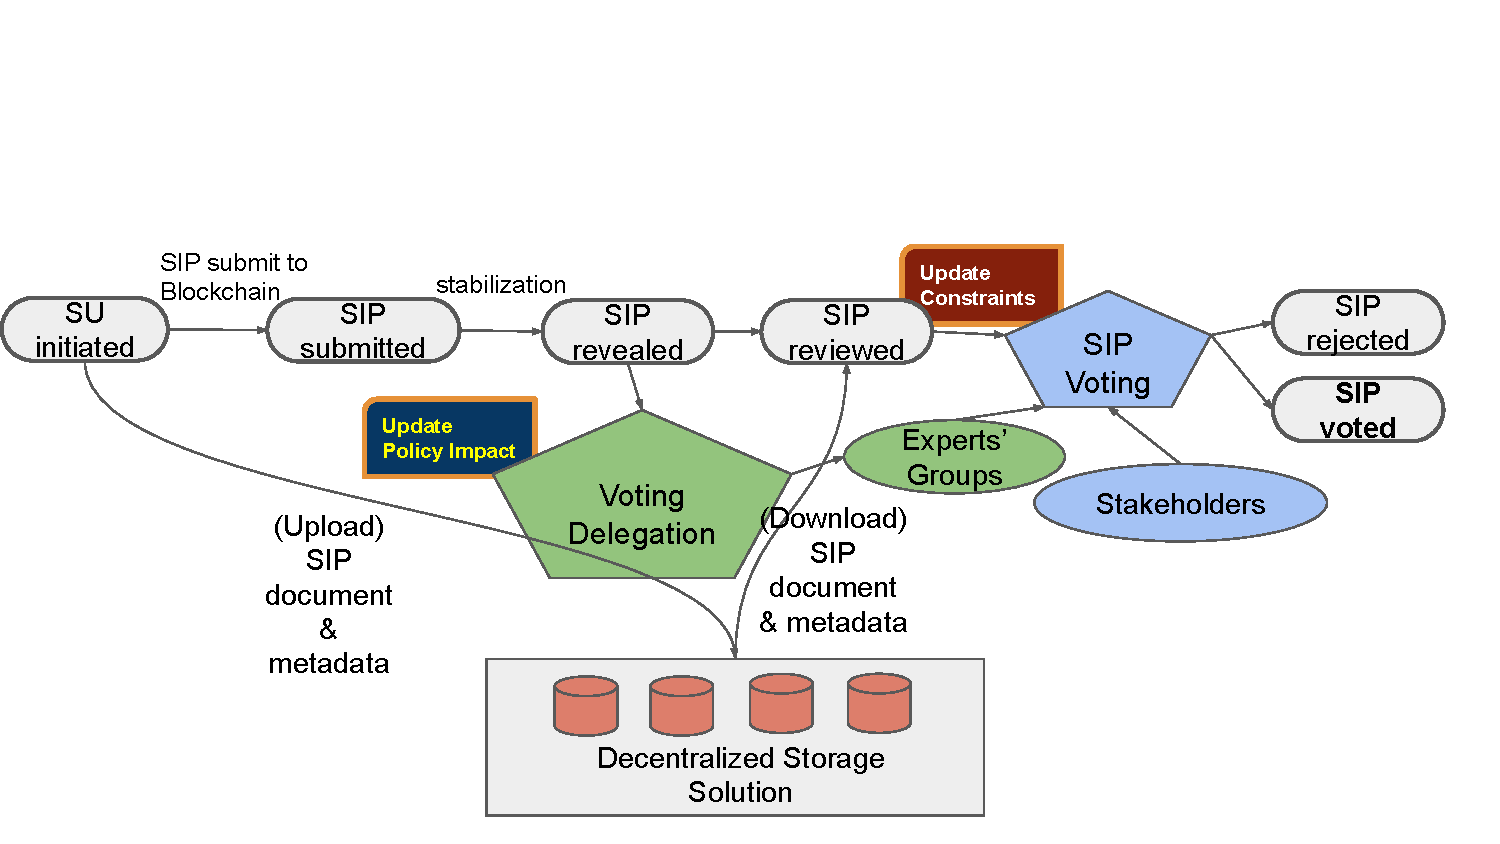
\includegraphics[width=1.0 \columnwidth,keepaspectratio]{figures/ideation_phase.pdf}
    \label{ideation}
\end{figure}
In the decentralized setting, a SU starts its life as an idea for improvement of the blockchain system, which is recorded in a human readable simple text document, called the \emph{SIP (Software  \footnote{\say{Software} and \say{System} are two terms that could be considered equivalent for the scope of this paper and we intend to use them interchangeably. For example, a SIP could also stand for a System Improvement Proposal} Improvement Document)}. The SU life starts by submitting the corresponding SIP to the blockchain by means of a special fee-supported transaction. Any stakeholder can potentially submit a SIP and thus propose a SU. 

A SIP includes basic information about a SU, such as the title, a description, the author(s) etc. Its sole purpose is to justify the necessity of the proposed software update and try to raise awareness and support from the community of users. A SIP must also include all necessary information that will enable the SU validation against previous SUs (e.g., update dependencies or update conflict issues), or against any prerequisites required, in order to be applied.

A SIP is initially uploaded to some external (to the blockchain system) \emph{decentralized storage solution} and a hash id is generated, in order to uniquely identify it. This is an abstraction to denote a not centrally-owned storage area, which is content-addressable, i.e., we can access stored content by using the hash of this content as an id. %A change in the content will produce a different hash and therefore this will correspond to a different id and thus to different stored content. 
This hash id is committed to the blockchain in a two-step approach, following a hash-based commitment scheme, in order to preserve the rightful authorship of the SIP.

Once the SIP is revealed a voting period for the specific proposal is initiated. Any stakeholder is eligible to vote for a SIP and the voting power will be proportional to his/her stake. Votes are specialized fee-supported transactions, which are committed to the blockchain.

%Note that since a SIP is a document justifying the purpose and benefit of the proposed software update, it should not require in general sufficient technical expertise, in order for a stakeholder to review it and decide on his/her vote. However, in the case that the 
In the case that the evaluation of a SIP requires greater technical knowledge, then a voting delegation mechanism exists. This means that a stakeholder can delegate his/her voting rights to an appropriate group of experts but also preserving the right to override the delegate's vote, if he/she wishes. 

%The delegation mechanism will also be used in order to implement the concept of an \emph{update policy} that will be described in a later section and enables different activation speeds for a SU depending on its type (e.g., a bug-fix versus a change request, a SU that has a consensus protocol impact versus a no-impact one, etc.). For all these, special \emph{delegation groups} will be considered, as we will discuss in the relevant section. A SIP after the voting period can either be voted or rejected. Details on the voting and delegation protocols can be found in the relevant section.

%Note that in the decentralized approach the ideation phase could very well be implemented by a treasury system (e.g., similar to the one proposed by Bingsheng et al. \cite{treasury}). A treasury is a decentralized and secure system aimed at the maintenance of a blockchain system that allows the submission of proposals (i.e., candidate projects) for improvement of the system. These proposals go through a voting process, in order to select the surviving ones. More importantly, the system is supported by a funding mechanism, where funds raised are stored in the treasury. These funds are used for funding the approved projects. Implementing the ideation phase with a treasury system, would enable additionally the appropriate management of the funding of each SU.

\subsection{Implementation}
%The voting of a SIP is the green light signal for entering the implementation phase. This is the period where the actual implementation of a SIP takes place. So one could very roughly imagine this phase as a box, where a SIP comes in as input and source-code implementing the SIP comes out as output.

%\paragraph{Scope of this phase.}
The scope of this phase is twofold: a) to develop the source-code changes that implement a specific voted SIP and b) to execute a second voting delegation round, in order to identify the experts that will approve the new source-code. At the end of this phase, the developer creates a bundle comprising the new source-code, the accompanied metadata and optionally produced binaries, which we call an \emph{update proposal (UP)}. The newly created UP must be submitted for approval, in order to move forward.

%\paragraph{Centralized approach.}
%In the centralized setting, it is typical (in the context of an open source software development model), when a developer wants to implement a change, first to download from a centrally-owned code repository the version of the source-code that will be the base for the implementation and then, when the implementation is finished, to upload it to the same code repository and submit a \emph{pull-request}. The latter is essentially a call for approval for the submitted code. The central authority responsible for the maintenance of the code-base, must review the submitted code and decide, if it will be accepted, or not. Therefore, in the centralized approach the implementation phase ends with the submission of a pull-request.

%\paragraph{Decentralized approach}
The decentralized alternative for the implementation phase is identical to its centralized counterpart as far as the development of the new code is concerned. However, in the decentralized setting, there exist these major differences:
a) there is not a centrally-owned code repository to maintain the code-base (since there is not a central authority responsible for the maintenance of the code), b) a delegation process is executed, in parallel to the implementation, as a preparation step for the (decentralized) approval phase that will follow and c) the conceptual equivalent to the submission of a pull-request (i.e., a call for approval by the developer to the code maintainer authority) must be realized.

\begin{figure}[h!] %[H]
    \caption{The implementation phase.}
    \centering
    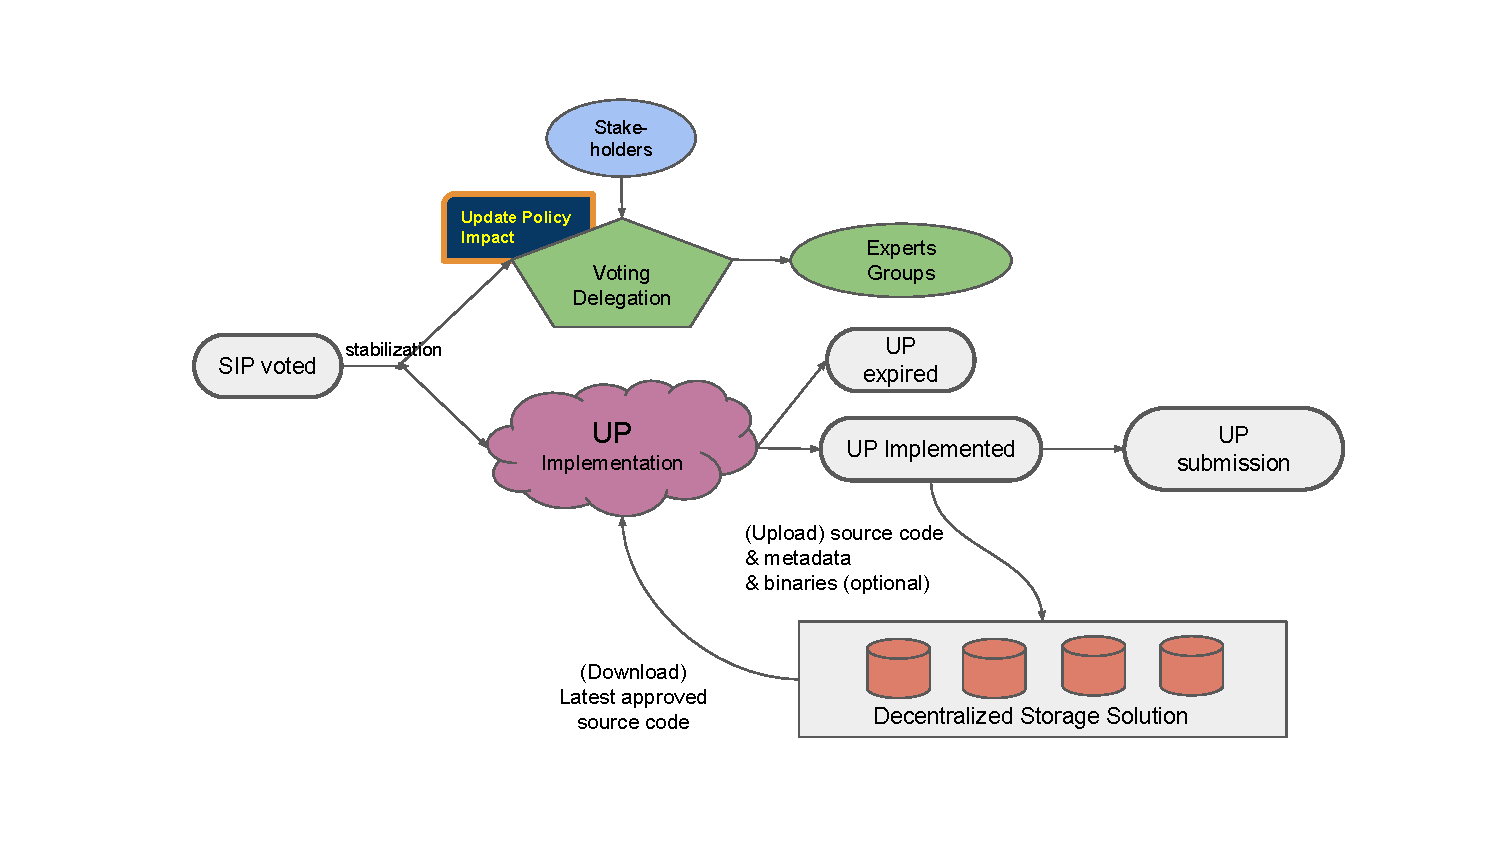
\includegraphics[width=1.0 \columnwidth,keepaspectratio]{figures/implementation_phase.pdf}
    \label{implementation}
\end{figure}

%In Figure \ref{implementation}, we depict the decentralized implementation phase. Similar to the centralized case, the implementation of a change must be based on some existing code, which we call the base source code and the developer must download locally, in order to initiate the implementation. However, in the decentralized setting there is not a centrally-owned code repository. All the approved versions of the code are committed into the blockchain (i.e., only the hash of the update code is stored on-chain). Therefore, we assume that the developer finds the appropriate (usually the latest) approved base source code in the blockchain and downloads it locally, using the link to the developer-owned code repository provided in the UP metadata. We abstract this code repository in Figure \ref{implementation} with the depicted decentralized storage solution. This conceptually can be any storage area that is not centrally-owned; from something very common, as a developer-owned Github repository to something more elaborate as a content-addressable decentralized file system.

In Figure \ref{implementation}, we depict the decentralized implementation phase. All the approved versions of the code are committed into the blockchain (i.e., only the hash of the update code is stored on-chain). Therefore, we assume that the developer finds the appropriate (usually the latest) approved base source code in the blockchain and downloads it locally, using the link to the developer-owned code repository provided in the UP metadata. We abstract this code repository in Figure \ref{implementation} with the depicted decentralized storage solution. This conceptually can be any storage area that is not centrally-owned; from something very common, as a developer-owned Github repository to something more elaborate as a content-addressable decentralized file system.

It is true that the review of source code is a task that requires extensive technical skills and experience. Therefore, it is not a task that can be assumed by the broad base of the stakeholders community. A voting delegation mechanism at this point must be in place, to enable the delegation of the strenuous code-approval task to some group of experts. 
%In a similar logic with the delegation process, within the ideation phase, discussed above, the delegation process could be leveraged to implement different update policies per type of software update.

%As we have seen, the voting approval of a SIP signals the beginning of the implementation phase for this SIP. 
%The SIP has an estimated implementation elapsed time that was included in the SIP metadata, submitted along with the SIP at the ideation phase. This time period, increased by a contingency parameter, will be the available time window for a SIP to be implemented. 
%Upon the conclusion of the implementation, a bundled (source code and metadata) UP is created. The UP must be uploaded to some (developer-owned) code repository and a content-based hash id must be produced that will uniquely identify the UP. This hash id will be submitted to the blockchain as a request to approval. This is accomplished with a specialized fee-supported  transaction, which represents the decentralized equivalent to a pull-request. SIPs that fail to be implemented within the required time framework (explicitly stated in the SIP metadata), will result to expired UPs and the SIP must be resubmitted to the ideation phase, as a new proposal. The UP submission transaction signals the entering into the approval phase.

Upon the conclusion of the implementation, the UP must be uploaded to some (developer-owned) code repository and a content-based hash id must be produced that will uniquely identify the UP. This hash id will be submitted to the blockchain as a request to approval. This is accomplished with a specialized fee-supported  transaction, which represents the decentralized equivalent to a pull-request.

\subsection{Approval}

%\nnote{The voter at this phase votes for three things: a) for the correspondence of the source code to the CIP (i.e., authenticity testing / security auditing), b) For the inclusion from the new source code of all previous approved UPs (i.e., regression testing), c) The correctness of the new code (i.e., testing)}

%\nnote{If there is also a binary upload for a specific platform for a UP, then the approval must vote for the authenticity and safety of the binaries as well. This might require a re-delegation to a specialized team for the specific platform. So this could be a separate vote}

%\paragraph{Scope of this phase.}
%The submission of an UP to the blockchain, as we have seen, is the semantic equivalent to a pull-request, in the decentralized approach. It is a call for approval. Indeed, the 
The main goal of the approval phase is to approve the proposed new code; but what exactly is the approver called to approve for? The submitted UP, which as we have seen, is a bundle consisting of source code, metadata and optionally produced binaries, must satisfy certain properties, in order to be approved:
\begin{itemize}
\item
\emph{Correctness and accuracy.} The UP implements correctly (i.e., without bugs) and accurately (i.e., with no divergences) the changes described in the corresponding voted SIP.

\item \emph{Continuity.} Nothing else has changed beyond the scope of the corresponding SIP and everything that worked in the base version for this UP, it continues to work, as it did (as long as it was not in the scope of the SIP to be changed).

\item \emph{Authenticity and safety.} The submitted new code is free of any malware and it is safe to be downloaded and installed by the community; and by downloading it, one downloads the original authentic code that has been submitted in the first place.

\item \emph{Fulfillment of update constraints.} We call the dependencies of an UP to other UPs, the potential conflicts of an UP with other UPs and in general all the prerequisites of an UP, in order to be successfully deployed, \emph{update constraints}. The fulfillment, or not, of all the update constraints for an UP, determines the feasibility of this UP.
\end{itemize}

%%\paragraph{Centralized approach.}
%From the centralized approach perspective the above properties of the new code that the approver has to verify and approve are not uncommon. In fact, one could argue that these are the standard quality controls in any software development model. The first property has to do with testing; testing that verifies that the changes described in the SIP have been implemented correctly and accurately. In the centralized approach this means that the main maintainer of the code has to validate that the new code successfully passes specific test cases, either by reviewing test results, of executed test cases, or by running tests on his/her own. Regardless, of the testing methodology or type of test employed (unit test, property-based test, system integration test, stress test etc.), this is the basic tool that helps the central authority to decide on the correctness and accuracy of the new code. 
%
%The second property for approving the new code has to do with not breaking something that used to work in the past. In software testing parlance, this is known as regression testing. Again, in the centralized approach, it is the main maintainer's responsibility to verify the successful results of regression tests run against the new code. 
%
%The third property has to do with the security of the new code and the authenticity of the downloaded software. The former calls for the security auditing of the new code. The latter, in the centralized case, is easy. Since, there is a trusted central authority (i.e., the main code maintainer), the only thing that is required, is for this authority to produce new binaries based on the approved source code, sign them and also the source code with his/her private key and distribute the signed code to the community. Then, the users only have to verify that their downloaded source code, or binaries, has been signed by the trusted party and if yes, then to safely proceed to the installation.
%
%Finally, the last property that has to be validated by the approver pertains to the fulfillment of the update constraints. All the prerequisites of an UP must be evaluated and also the potential conflicts triggered by the deployment of an UP must be considered. For example, an UP might be based on a version of the software that has been rejected; or, similarly, it might be based on a version that has not yet been approved. Moreover, it might require the existence of third party libraries that it is not possible to incorporate into the software (e.g., they require licenses, or are not trusted). Then, we have the potential conflicts problem. What if the deployment of an UP cancels a previously approved UP, without this cancellation to be clearly stated in the scope of the corresponding SIP? All these are issues that typically a code maintainer takes into consideration, in order to reach at a decision for a new piece of code.

%\paragraph{Decentralized approach.}
Once more, the essential part that differentiates the decentralized from the centralized approach is the lack of the central authority. All the properties that have to be validated basically remain the same but in this case the approval must be a collective decision.
The approval phase in the decentralized approach is depicted in Figure \ref{approval}.

\begin{figure}[h!] %[H]
    \caption{The approval phase.}
    \centering
    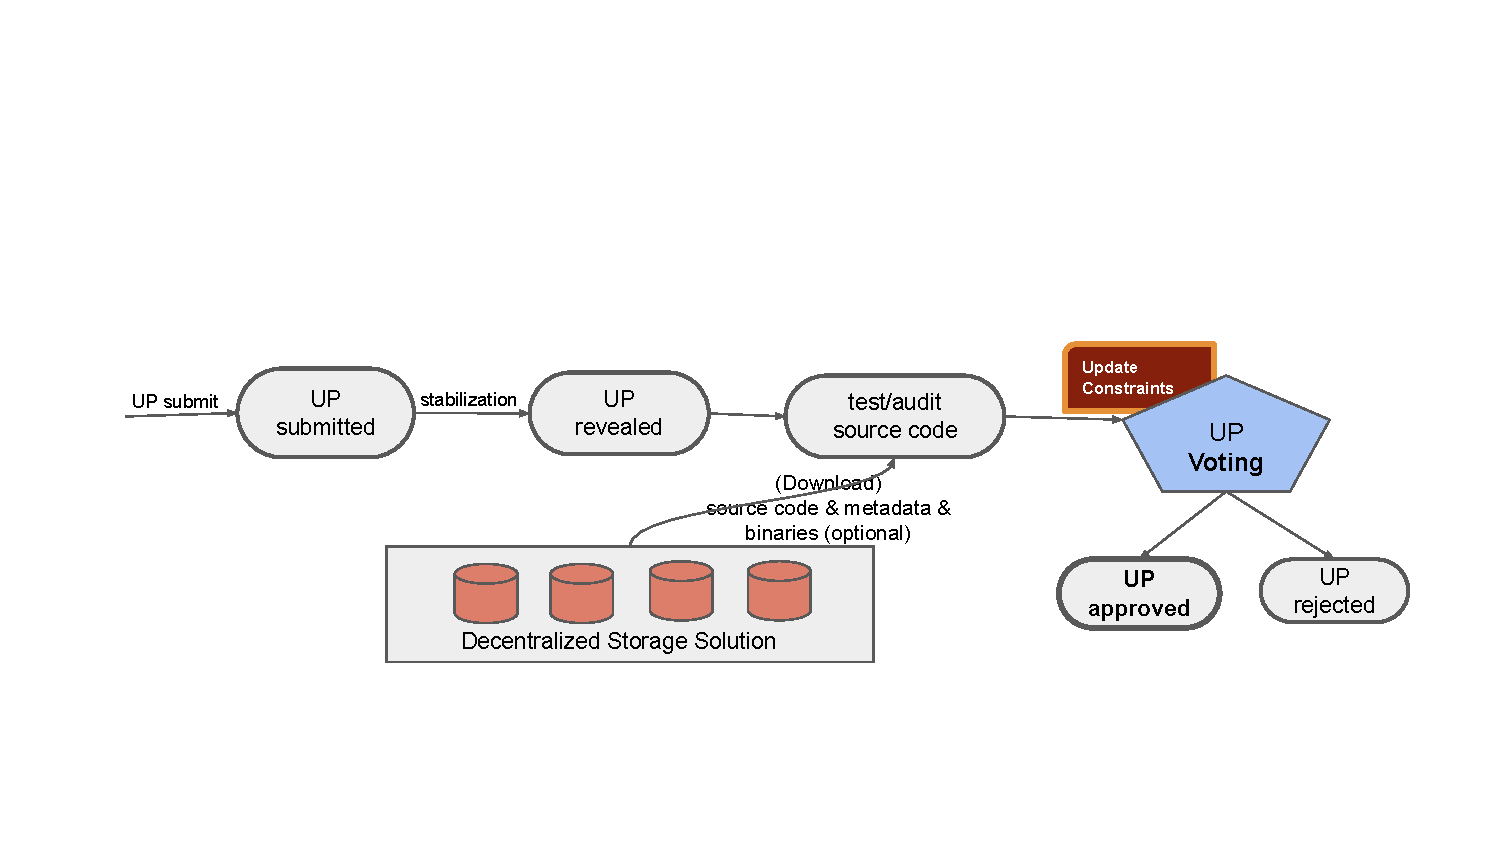
\includegraphics[width=1.0 \columnwidth,keepaspectratio]{figures/approval_phase.pdf}
    \label{approval}
\end{figure}

%The approval phase in the decentralized approach is depicted in Figure \ref{approval}. As we have seen, an UP is a bundle consisting of source code, update metadata and optionally binaries produced from the source code, aiming at a specific platform (e.g., Windows, Linux, MacOS etc.). The update metadata have to include basic information about the update, its justification, they have to clearly state all update constraints and finally declare the type of the change (e.g., bug-fix, or change request, soft/hard fork etc.)
% and priority, in order to enable the appropriate \emph{update policy} (we will return to these concept in the relevant section). 
%The UP bundle is uploaded to some developer-owned code repository and a unique hash id, from hashing the content of the UP is produced. This UP hash id is submitted to the blockchain, along with a link to the code repository.

%Similar to the ideation phase (where the corresponding SIP was submitted), the submission of a UP is a special fee-supported transaction that can be submitted by any stakeholder. The UP is committed to the blockchain following again a hash based commitment scheme, in order to preserve the rightful authorship of the UP.

Once the UP is revealed the delegated experts (remember the delegation that took place during the implementation phase) for this UP, will essentially assume the role of the main code maintainer that we typically see in a centralized setting. In other words, they have to download the source code, metadata and possible binaries and validate the aforementioned properties. %The tools (e.g., testing) that the experts have available for doing the validation are no different than the tools used by the main maintainer in the centralized approach. Moreover, if binaries for a specific platform have been uploaded by the UP submitter, then the delegated experts must go through the process of reproducing a binary from the source code and verifying that it matches (based on a hash code comparison) the one submitted. If not, then the submitted binary must be rejected and this will cause a rejection of the UP as a whole. So there must be some extra caution when binaries are submitted along with source code, since the metadata need to include sufficient information for the approver to be able to reproduce the same binaries per platform.

%Therefore the revealing of a UP, initiates a voting
The revealing of a UP, initiates a voting period for the specific proposal, in which the delegated experts must validate \emph{all} the UP properties posed and approve, or reject it, with their vote. Any stakeholder is eligible to vote for an UP and the voting power will be proportional to his/her stake. If a stakeholder wishes to cast a vote, although he/she has already delegated this right to an expert, then this vote will override the delegates vote. Votes are specialized fee-supported transactions, which are committed to the blockchain. %We will return to the voting protocol in the relevant section.

%One final note is that, as we have described, the decentralized approval phase that we propose, entails transaction fees. This means that the approval phase is not so flexible from a practical perspective,  as to be used iteratively (although technically this is possible). In other words, to reject an UP, then fix some bugs and upload a new version for review etc. An UP rejection means that a resubmission must take place, with all the overhead that this entails (transaction fees, storage costs, a new voting must take place, etc.). This is a deliberate design choice that guards the system against DoS attacks. From a practical perspective though, it means that the submitted UPs must be robust and thoroughly tested versions of the code, in order to avoid the resubmission overhead. We do not want to pollute the immutable blockchain history with intermediate trial-and-error UP events.

\subsection{Activation}

%\paragraph{Scope of this phase.}
The final phase in the lifecycle of a software update, depicted in Figure \ref{lifecycle}, is the activation phase. This is a preparatory phase before the changes actually take effect. It is the phase, where we let the nodes do all the manual steps necessary, in order to upgrade to an approved UP and at the end, send a signal to their peers that they are ready for the changes to be activated. Thus, the activation phase is clearly a signaling period. Its primary purpose is for the nodes to signal upgrade readiness, before the actual changes take effect (i.e., activate). 

Why do we need such a signaling period in the first place? Why is not the approval phase enough to trigger the activation of the changes? The problem lies in that there are manual steps involved for upgrading to the new software, such as downloading and building the software from source code, which entail delays that are difficult to foresee and standardize. This results into the need for a synchronization mechanism between the nodes that upgrade concurrently. The lack of such a synchronization between the nodes, prior to activation, might cause a chain split. %This synchronization mechanism exactly is the activation phase and for this, it is considered very important. 

Clearly, the activation phase is not aimed as a re-approval phase for the UP. It is there to allow a smooth incorporation of the software update into the network. Therefore it becomes relevant only for those UPs that impact the consensus and can risk a chain split. For UPs that don't impact the consensus (e.g., a code refactoring, or some short of optimization, or even a change in the consensus protocol rules, which is a velvet fork \cite{velvet}) there is essentially no need for an activation phase and the change can activate, as soon as the software upgrade takes place.

%%\paragraph{Centralized approach.}
%Traditionally, when a software update needs to be activated and it is known that it is likely to cause a chain split, a specific target date, or better, a target block number is set by the central authority, so that all the nodes to get synchronized. Indeed, this is a practice followed by Ethereum \cite{ethereum}. All major releases have been announced enough time before the activation, which takes place when a specific block number arrives (i.e., the corresponding block is mined). All nodes must have upgraded by then, otherwise they will be left behind. In Bitcoin \cite{bitcoin}, there also exists a signaling mechanism\footnote{see BIP-9 at https://github.com/bitcoin/bips/blob/master/bip-0009.mediawiki}. In this case, the activation takes place, only if a specific percentage of blocks (95\%) within a retargeting period of 2016 blocks, signal readiness for the upgrade. 

%\paragraph{Decentralized approach.}
Once the UP approval result has been buried under a sufficient number of blocks (i.e., the stabilization period passes), then the activation period is initiated. In Figure \ref{activation}, we depict the activation period in the decentralized setting.

\begin{figure}[h!] %[H]
    \caption{The activation phase.}
    \centering
    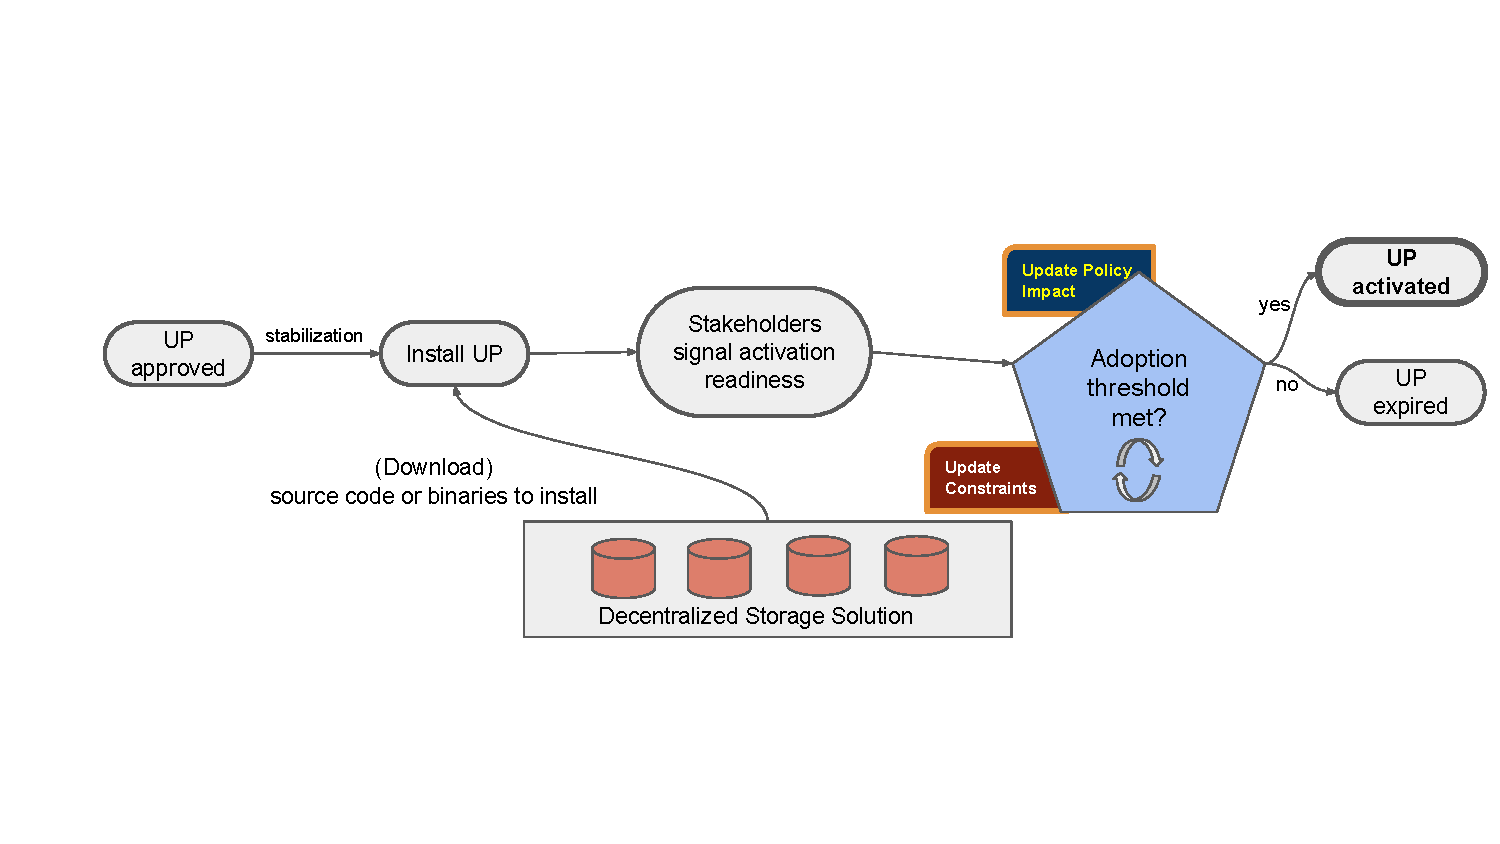
\includegraphics[width=1.0 \columnwidth,keepaspectratio]{figures/activation_phase.pdf}
    \label{activation}
\end{figure}

%The first step in the activation phase is the installation of the software update. Typically, as soon as the UP approval is stabilized in the blockchain, the GUI of the client software (e.g., the wallet) prompts the user to download and install the update, using the link that accompanies the UP. If in the UP bundle there exists an approved binary, then the user can download and install this, otherwise the user must download the approved source code. In the latter case, there exist an extra step of producing the binary code from the source code. In any case, it is important to note that the new software is just installed but not activated. It will remain in a latent state until the actual activation takes place.
The first step in the activation phase is the installation of the software update. It is important to note that the new software is just installed but not activated. It will remain in a latent state until the actual activation takes place.

For the nodes participating in the consensus protocol the installation of a software update means that they are ready to activate, but wait to synchronize with their other peers. To this end, they initiate signaling. This means that every new block issued will be stamped with the new version of the software, signifying their readiness for the new update.

When the first block with the new version appears, we enter the adoption period for the specific UP. During the adoption period the following conditions have to be met, in order for the activation to take place: a) The number of blocks with a signal must exceed a specific threshold, b) the update constraints for the specific UP must be fulfilled and c) the adoption time period must not be exceeded, otherwise the UP will become expired. The blocks generated in a proof-of stake protocol are proportional to the stake and therefore, we can assume that the signaling mechanism is also proportional to the stake. 
When the first block with the new version appears, we enter the adoption period for the specific UP. The blocks generated in a proof-of stake protocol are proportional to the stake and therefore, we can assume that the signaling mechanism is also proportional to the stake. Once the stake threshold from the signals of the new blocks is reached, then the changes can take effect.
%We can also assume that the honest stake majority, will follow the protocol and eventually will upgrade and thus signal this event with their generated blocks. This means that the minimum expected percent of signals (i.e., the activation threshold) cannot be other that the minimum percent of honest stake majority required by the proof-of-stake consensus protocol. Of course, as we have noted above, for changes that don't impact the protocol, the activation threshold could be zero; meaning that even if only one node upgrades, then the changes can be immediately activated.

%Moreover, the adoption time period is not fixed for all UPs. It varies based on the type of the change, which is something recorded in the UP metadata. One size does not fit all, and this is indeed true for the adoption time period of UPs. For example, major updates that require a lot of manual steps, or significant build time, or even hardware upgrade, should be adopted in a sufficient period of time, while small updates should be activated more swiftly.

Finally, before the actual activation of a change, the validation of all the update constraints must take place once more. This is true, although we make the assumption that from the approval phase all relevant update constraints' issues (like conflicts, or dependencies) have been considered. The fact that the adoption period might require significant time for a UP, whose update constraints were fulfilled at the approval phase, while concurrently there are other UPs that become activated, means that the conditions might have changed and the update constraints must be reevaluated to make sure that no problems will arise upon activation of a UP.
